\section{Introduction}\label{sec:intro}

Feature engineering matters for tabular prediction: a few ratios, thresholds, or interactions can change the problem a downstream model sees, so recent work uses large language models (LLMs) to propose them. CAAFE has an LLM write feature code \citep{hollmann2023caafe}, FeatLLM parses LLM rules into binary features \citep{han2024featllm}, and others serialize rows as text for direct prediction \citep{hegselmann2023tabllm} or optimize feature programs with LLMs \citep{abhyankar2026llmfe,nam2024octree}. From a data-centric perspective, all of these systems are automated data-preparation tools: they change the feature representation that a downstream model sees, and their value should be measured with the same care as any other change to the data.

Two mechanisms are easy to conflate. A schema-level call writes deterministic formulas such as ratios or indicators once, at no per-row inference cost. An instance-level call reads each row and emits a judgment: flexible but expensive, slow, and hard to audit.

We ask whether LLM-generated formulas carry real semantic signal or merely add columns, and whether per-row judgments add anything beyond them. These are benchmarking questions about a data-preparation step: the object under evaluation is the feature representation, the unit of analysis is the dataset, and each control holds the data fixed except for the property under test, following the data-centric view that benchmarks data preparation itself \citep{zha2025datacentric,mazumder2023dataperf,tschalzev2024datacentric}. Because popular public tables are in the models' training data \citep{bordt2024elephants}, the benchmark also needs contamination controls.

The most robust result is a semantic control, not the raw-to-formula comparison: correct formula features consistently beat the same features with generated columns independently row-permuted. On 49 datasets and four schema generators it is significant after multiple-comparison correction for all four downstream models, largest for logistic regression (LR) and \(k\)-nearest neighbors (KNN), smaller for tree ensembles, and present for every generator, under column anonymization, and on six post-cutoff tables. Much of this gap is generic to any valid expression over the same columns; the generator-specific remainder is small but consistent for LR and KNN, smaller for RF, and absent for XGBoost. Direct gains over raw features are small and model-dependent, no generator, LLM or classical automated feature engineering (AutoFE), helps tree ensembles, and per-row judgments add essentially nothing beyond formulas.

Contributions:

\begin{itemize}
\item
  A documented two-tier benchmark: 49 OpenML classification datasets (10 core, 39 expansion) with recorded identifiers, versions, and licences (Appendix~\ref{app:datasets}), evaluating schema-level formulas and per-row judgments from four generators under one protocol.
\item
  A benchmarking method for feature generators: a column-permutation control that preserves marginal distributions and feature count but breaks row alignment, paired with a count-matched random-expression control over the same columns and vocabulary (Section~\ref{sec:random-expression}).
\item
  Two contamination controls for public-table benchmarks: an anonymized-column control on the core datasets and a replication on six real datasets with provenance and licences (Appendix~\ref{app:postcutoff-data}) whose tables post-date the generators' training data (Section~\ref{sec:postcutoff}).
\item
  A negative result for per-row LLM judgments: on the ten core datasets they do not improve over zero-inference-cost deterministic formulas.
\item
  Classical AutoFE baselines (polynomial, OpenFE, autofeat) on the 49 datasets: search-based OpenFE matches the LLM formulas for LR and is at least as good for KNN; our contribution is the controlled decomposition, not a state-of-the-art generator.
\end{itemize}

\section{Related Work}\label{sec:related-work}

\paragraph{LLMs for tabular learning and feature engineering.}

LLMs serve tabular data as predictors and feature generators \citep{fang2024survey,hegselmann2023tabllm}: CAAFE, FeatLLM, and FELIX turn LLM-proposed transformations or rules into features \citep{hollmann2023caafe,han2024featllm,malberg2024felix}; later work searches over feature programs \citep{nam2024octree,abhyankar2026llmfe,gong2025evolutionary,zhang2025dynamic} or lets agents revise whole pipelines on Kaggle-derived benchmarks \citep{guo2024dsagent,hong2025datainterpreter,chi2024sela,jiang2025aide,li2024autokaggle,chan2025mlebench}. LLM generators favor simple operators at a cost in predictive performance \citep{kuken2024simple}, motivating our random-expression control over the same vocabulary (Section~\ref{sec:controls}). We isolate two mechanisms these systems bundle: deterministic formulas and per-row judgments.

\paragraph{Traditional automated feature engineering.}

Classical AutoFE builds and selects transformations without language-model semantics by composing primitives across linked tables \citep{kanter2015dfs}, searching or learning which transformations help \citep{khurana2016cognito,katz2016explorekit,nargesian2017lfe,khurana2018rl,zhu2022difer}, or filtering large candidate pools in stages \citep{horn2020autofeat,zhang2023openfe}. As they too add columns, they are natural baselines; we run polynomial interactions, OpenFE, and autofeat to completion on the same 49 datasets (Section~\ref{sec:classical}).

\paragraph{Evaluation across datasets.}

Cross-dataset comparisons use nonparametric tests, Wilcoxon signed-rank \citep{wilcoxon1945individual} for pairs and Friedman/Nemenyi \citep{friedman1937use} for rankings \citep{demsar2006statistical,garcia2010advanced}, and large benchmarks report per-dataset ranks or normalized scores rather than pooled scores \citep{grinsztajn2022tree,mcelfresh2023neural,erickson2025tabarena}. We follow suit: the dataset is the statistical unit; fold-level variation serves estimation only.

\paragraph{Permutation controls.}

Permuting labels \citep{ojala2010permutation} or single features \citep{breiman2001random,fisher2019all,altmann2010permutation,strobl2008conditional} tests for dependence on feature-label alignment rather than distributional artifacts, though unconditional test-time permutation forces extrapolation to unseen feature combinations \citep{hooker2021unrestricted}. Our control independently permutes each generated column before cross-validation, so the model is refitted on the permuted columns, not evaluated off-distribution. Beating the permuted copy rules out dimensionality, syntax, and marginal distributions as sole explanations; the random-expression control (Section~\ref{sec:controls}) asks how much of the gap any valid expression over the same columns produces.

\paragraph{Contamination and memorization in tabular LLM evaluation.}

Language models memorize training data \citep{carlini2023quantifying}, so test sets seen in pretraining inflate measured ability \citep{sainz2023nlp,xu2024benchmark}; detectors use guided completion \citep{golchin2024time} or post-cutoff problems \citep{roberts2024cutoff,white2025livebench}, and \citet{bordt2023testing,bordt2024elephants} show verbatim memorization of popular tabular datasets and higher few-shot performance on tables seen in training. We likewise use post-cutoff tables (Section~\ref{sec:postcutoff}) and anonymized schemas that hide column names and dataset identity (Section~\ref{sec:anon}); both controls are partial (Sections~\ref{sec:postcutoff} and~\ref{sec:limitations}).

\paragraph{Tabular benchmarks and data-centric evaluation.}

OpenML suites pin collections and versions \citep{vanschoren2014openml,bischl2021openml}; large comparisons show that conclusions depend on dataset population, evaluation protocol, and split design \citep{gorishniy2021revisiting,grinsztajn2022tree,mcelfresh2023neural,ye2024closer,erickson2025tabarena,rubachev2025tabred}. \citet{tschalzev2024datacentric} argue that dataset-specific feature engineering changes model rankings and belongs in the benchmark, as data-centric AI \citep{zha2025datacentric,liang2022advances} and DataPerf \citep{mazumder2023dataperf} do for data preparation; datasheets \citep{gebru2021datasheets} set the documentation standard of Appendices~\ref{app:datasets} and~\ref{app:postcutoff-data}. We treat LLM feature generation the same way: the benchmark is pinned to OpenML identifiers, versions, and licences, and each control varies one property.

\section{Evaluation Pipeline and Controls}\label{sec:method-the-dasef-pipeline}

The DASEF (Downstream-Aware Semantic Feature Engineering) pipeline (Figure~\ref{fig:pipeline}) has four steps: a schema-level LLM call on a column summary, formula materialization, optional per-row judgments, and count-matched and row-permutation controls scored with every schema run.

\begin{figure}[tbp]
\centering
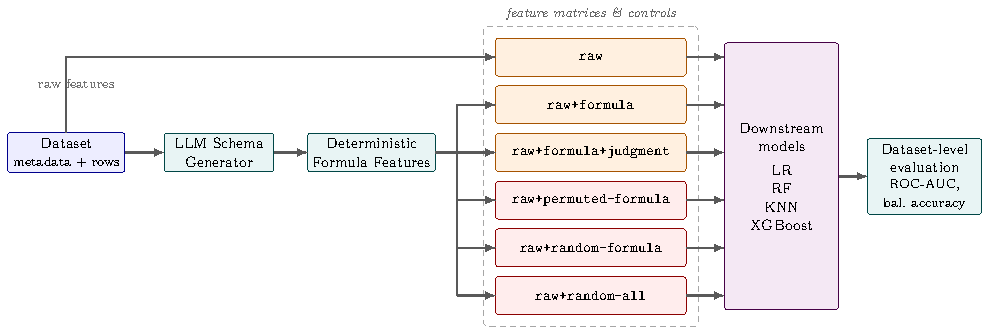
\includegraphics[width=\linewidth]{figures/fig1_pipeline.pdf}
\caption{Overview of the DASEF evaluation pipeline. Schema-level LLM calls generate deterministic formulas once per dataset; downstream evaluation compares raw features, formula features, optional per-row judgments, and controls that preserve feature count while removing semantic alignment. The count-matched random-expression control of Section~\ref{sec:controls} is evaluated alongside these matrices (not shown); the generator receives only the column-level summary of the design split, never rows.}\label{fig:pipeline}
\end{figure}


\subsection{Schema-level formula generation}\label{sec:schema-level-formula-generation}

For each dataset, a schema generator receives a column-level summary of a schema-design split: column names, dtypes, missing rates, mean/std/min/max for numeric columns or the ten most frequent values for categorical ones, and the class balance. No rows or row-level labels are sent. It returns a fixed schema of 12 features: deterministic formulas plus per-row judgment specifications (counts in Appendix~\ref{app:protocol-details}). Formulas are then applied to the evaluation rows without further LLM calls.

Four generators were evaluated: Claude Opus 4.7, Claude Sonnet 4.6, Gemini 3.1 Pro Preview, and GPT-5.5 Pro, each prompted for three model families: linear and support-vector-machine (linear/SVM), tree/ensemble, and distance-based KNN. The family labels are experimental conditions, not evidence of specialization: a downstream-awareness diagnostic on the core tier finds no reliable matched-family advantage (Section~\ref{sec:discussion}). Benchmark-wide analyses therefore use each generator's linear/SVM schema, averaged over the generators covering a dataset before testing; the core tier has all three families from all four generators (Appendix~\ref{app:core-families}).

\subsection{Per-row judgment generation}\label{sec:judgment}

The second component appends row-level LLM judgments, intended to capture what deterministic formulas cannot express. Judgments are the expensive component, since they need row-level LLM calls, and are harder to reproduce and audit, so their value is assessed only incrementally: \texttt{raw+formula} versus \texttt{raw+formula+judgment}. DeepSeek-Reasoner produced them in 25-row batches for all 120 core runs; Appendix~\ref{app:judgment-v4pro} reports a second judgment model, and the expansion tier has none (Appendix~\ref{app:protocol-details}).

\subsection{Controls}\label{sec:controls}

\paragraph{Column-permuted formula control.}

The strongest control keeps the materialized formula features but independently permutes each generated column across evaluation rows. This preserves the feature count and each column's exact marginal distribution but breaks row alignment; a column with row-aligned structure should beat its permuted copy. It tests row-aligned signal in the materialized feature, not whether the LLM invented it. Each column is permuted once over the whole evaluation split (seed 42) before cross-validation, so training and test folds are permuted jointly. Scoring uses the same folds, fold by fold, with one draw per schema run.

\paragraph{Random feature control.}

Random controls add uniform-noise columns (seeds 42 and 43) matched in count and declared value range (Appendix~\ref{app:protocol-details}) to the formula features (\texttt{raw+random-formula}) or to all schema features, judgment specifications included (\texttt{raw+random-all}). They test whether arbitrary added columns suffice, and are less stringent than permutation because they do not preserve formula syntax.

\paragraph{Random-expression control.}

For every (dataset, generator) cell of the linear/SVM benchmark, this control draws \(k\) random but valid expressions over the dataset's own columns from the vocabulary of the LLM formulas, with \(k\) the number of formula features in the cell's LLM schema and only design-split column statistics as input; five independent draws per cell are scored and averaged. Materialization, range clipping, folds, downstream models, and column permutation match the LLM formulas (Appendix~\ref{app:protocol-details}). It asks whether random valid expressions help over \texttt{raw}, how much of the aligned-versus-permuted gap they reproduce, and whether the LLM's choices beat random choices of the same size and vocabulary (\texttt{raw+formula} versus \texttt{raw+random-expression}; Section~\ref{sec:random-expression}).

\subsection{Evaluation protocol}\label{sec:protocol}

Datasets above 5,000 rows are capped to a stratified 5,000-row sample (seed 42). A stratified 30\% schema-design split follows (seed 42), and the remaining 70\% are the evaluation rows: 3,500 for capped datasets, 524 to 3,783 otherwise. Scores use 5-fold cross-validation (CV) with 2 repeats. The downstream models are logistic regression (LR; class-balanced, up to 2,000 iterations), random forest (RF; 300 trees, \(\sqrt{p}\) candidate features per split, balanced-subsample class weights), \(k\)-nearest neighbors (KNN; \(k = 15\)), and XGBoost \citep{chen2016xgboost} (300 trees, depth 4, learning rate 0.05, 0.9 row and column subsampling), with library defaults otherwise. Numeric columns are median-imputed and, for LR and KNN, standardized; categorical columns are mode-imputed and one-hot encoded. Six core datasets (adult income, bank marketing, car evaluation, electricity, phoneme, spambase) come from a local cache; in three of them (adult income, bank marketing, car evaluation) it stores the categorical columns as integer codes. The schema generators therefore saw these columns as integers and their formulas compute on the codes; before downstream modelling the columns are restored to categoricals, so the raw block is one-hot encoded as for every other dataset (Appendix~\ref{app:protocol-details}). The primary metric is one-vs-rest ROC-AUC, macro-averaged over classes for the 12 multiclass datasets; balanced accuracy is secondary.

On both tiers the schema summaries came from design splits of the full, uncapped dataset, so on capped datasets they also cover later evaluation rows. Only distributional statistics and the class balance were exposed, never row-level labels; Section~\ref{sec:leakage} bounds the effect (Appendix~\ref{app:protocol-details}).

Matrix variants:

\begin{itemize}
\item
  \texttt{raw}: preprocessed original features.
\item
  \texttt{raw+formula}: plus the LLM formulas.
\item
  \texttt{raw+formula+judgment}: plus per-row judgments (core tier only).
\item
  \texttt{raw+permuted-formula}: plus the formulas with each generated column row-permuted.
\item
  \texttt{raw+random-formula}: plus uniform noise count- and range-matched to the formulas.
\item
  \texttt{raw+random-all}: plus uniform noise matched to all schema features.
\item
  \texttt{raw+random-expression}: plus count-matched random valid expressions (linear/SVM cells only), also scored permuted.
\end{itemize}

\subsection{Statistical analysis}\label{sec:statistical-analysis}

The statistical unit is the dataset. For each dataset, downstream model, metric, and matrix pair, fold-level scores are averaged within each schema run, then over the generators covering the dataset (four for 34 of the 49 datasets; Section~\ref{sec:datasets}); paired differences are then taken per dataset. Paired \(p\)-values are exact two-sided Wilcoxon signed-rank tests over the dataset-level differences, ties excluded, with Holm-Bonferroni correction over the four downstream models (family size four, within each metric and contrast) reported alongside. Cliff's \(\delta\) is the one-sample form \((wins - losses)/N\) against zero; 95\% confidence intervals (CI) for mean differences are percentile bootstrap intervals over datasets (10,000 resamples). Rankings use the Friedman test with the Nemenyi post-hoc critical difference \citep{demsar2006statistical}. Core-tier-only analyses (per-row judgments, schema families, the anonymized control) have ten datasets and sit at the Wilcoxon floor, where the smallest attainable two-sided \(p\) is \(0.002\) for a 10/10 sweep; they are reported uncorrected as supporting evidence. A global Benjamini-Hochberg check over all 48 tests of Tables~\ref{tab:semantic-direct} and~\ref{tab:random-expression} leaves every cell reported as significant below \(q = 0.05\); Appendix~\ref{app:protocol-details} gives the Holm-over-48 picture.

The contrasts are

\begin{align}
\Delta_{\mathrm{formula}}  &= s(\texttt{raw+formula}) - s(\texttt{raw}), \label{eq:formula}\\
\Delta_{\mathrm{judgment}} &= s(\texttt{raw+formula+judgment}) - s(\texttt{raw+formula}), \label{eq:judgment}\\
\Delta_{\mathrm{semantic}} &= s(\texttt{raw+formula}) - s(\texttt{raw+permuted-formula}), \label{eq:semantic}
\end{align}

where \(s( \cdot )\) is the cross-validated score for a fixed dataset, downstream model, and metric. The main claim is about \(\Delta_{\mathrm{semantic}}\), not \(\Delta_{\mathrm{formula}}\): a feature can encode real semantic structure yet not improve a high-capacity model over raw inputs.

\section{Benchmark Construction and Experimental Setup}\label{sec:experimental-setup}

\subsection{Datasets: a two-tier benchmark}\label{sec:datasets}

The two tiers are listed in Appendix~\ref{app:datasets} (Table~\ref{tab:datasets}).

\paragraph{Core tier (10 datasets).}

Ten OpenML \citep{vanschoren2014openml} classification datasets span low-feature medical and behavioral, categorical symbolic, business and socioeconomic, signal-processing, and higher-dimensional numeric/text-derived tasks: adult income, bank marketing, blood transfusion, car evaluation, credit-g, electricity, phoneme, pima diabetes, QSAR biodegradation, and spambase. Every core dataset has schemas from all four generators and all three families (12 schema runs), per-row judgment matrices, and the anonymized-column control. Three of the six locally cached core datasets (Section~\ref{sec:protocol}) are variants of the listed OpenML table: bank marketing is the 20-feature, 41,188-row UCI bank-additional variant rather than the 16-feature OpenML 1461 version, electricity is a 7-feature, 38,474-row variant of OpenML 151 without the \texttt{day} column, and adult income is the 45,222-row complete-case version of OpenML 1590.

\paragraph{Expansion tier (39 datasets).}

The expansion tier adds every dataset from a pool of 42 further OpenML classification datasets, configured for a planned larger study, with a valid cached linear/SVM-family schema from at least one generator and a successful stratified 30/70 split. Three are excluded: \texttt{advanced\_iot\_dataset} and \texttt{letter}, where every generator response failed validation, and \texttt{nursery}, whose single-member class the stratified split rejects. Each expansion dataset has the linear/SVM schema of every generator that produced one: 24 of the 39 are covered by all four generators, seven by three, six by two, and two by one (Gen.\ column of Table~\ref{tab:datasets}). This tier has no judgment features and only the linear/SVM family, so judgment, family, and anonymization analyses use the core tier only and formula-mechanism analyses all 49 datasets. In 13 schema cells on seven datasets whose column names are not valid Python identifiers, the generator saw column names sanitized to valid identifiers, and the same renaming is applied to the evaluation rows before materialization (Appendix~\ref{app:provenance} lists the cells).

\subsection{Scale of evaluation}\label{sec:scale-of-evaluation}

The formula evaluation covers 251 schema runs, 120 on the core tier (4 generators \(\times\) 3 families \(\times\) 10 datasets) and 131 on the expansion tier, each with five matrix variants (six on the core tier, where the judgment matrix is added), four downstream models, and 5-fold \(\times\) 2-repeat cross-validation, roughly 55,000 fold-level downstream evaluations; the random-expression control adds two matrices for each of five random draws in each of the 171 linear/SVM cells, a further 68,400. Each schema run is one generator call cached by prompt hash; the expansion schemas were evaluated offline from that cache, so no schema was selected or edited after its evaluation was known. The judgment columns alone reach ROC-AUC 0.66 with logistic regression, so they carry signal; Section~\ref{sec:per-row-judgments-add-no-reliable-value-beyond-formulas} shows this signal is redundant with \texttt{raw+formula}. Appendix~\ref{app:provenance} reports the judgment audit, response accounting, truncated schemas, and a constant-column scan.

\subsection{Prospective versus cached schema generation}\label{sec:leakage}

Schemas were generated from design-split summaries of the uncapped table, so on capped datasets of both tiers the summarized rows overlap the evaluation rows (Section~\ref{sec:protocol}). A leakage-equivalence check bounds this overlap: on 54 overlapping cells, the raw-to-formula deltas from cached and prospective evaluation of the same schemas differ by 0.0050 in mean absolute value and by \(+0.0023\) signed (cached minus prospective; Appendix~\ref{app:provenance}).

\subsection{Reproducibility}\label{sec:reproducibility}

Random seeds are 42 for the row cap, the design split, cross-validation, and permutations, and 43 for the random-all control. Checked-in scripts regenerate the classical baselines (Section~\ref{sec:classical}), the mechanism case study (Appendix~\ref{app:mechanism}), every control, and every aggregate, table, and figure offline from the cached schemas and stored matrices. Table~\ref{tab:models} (Appendix~\ref{app:provenance}) lists generator API identifiers, settings, and query dates, and the appendix records compute. A final audit found and fixed three formula-evaluator defects (a column named like a numpy function was shadowed by that function, \texttt{category}-typed columns were coerced so that string comparisons or arithmetic on them became silently constant, and narrow integer columns overflowed inside sums and products); every stored run was re-materialized and affected runs re-evaluated with the corrected evaluator, which produced every number reported here.

\paragraph{Data and code availability.}

Code, cached schemas and raw generator responses, per-fold scores, the benchmark definition, per-dataset provenance records (\texttt{dataset\_provenance.csv}), and the scripts regenerating every table and figure are in the supplementary material and at \url{https://github.com/prasad-yashdeep/dasef-tabular-research} (release \texttt{v1.1-dmlr-submission}); the stored feature matrices and the per-row judgment outputs are release assets there. Code is released under the MIT licence and derived artifacts (schemas, responses, scores, statistics, generated columns) under CC BY 4.0, except that artifacts derived from the two CC BY-NC post-cutoff tables carry the same non-commercial restriction; raw dataset columns embedded in the released matrices and the cached tables remain under their sources' terms. A datasheet-style description accompanies the supplement; the intended use is controlled evaluation of feature-generation tools for tabular classification under the controls of Section~\ref{sec:controls}, not training deployed models on the generated features. Appendix~\ref{app:provenance} covers table licences and maintenance.

\section{Results}\label{sec:results}

\subsection{Formula features encode semantic structure}\label{sec:semantic}

Across the 49 datasets, correct formulas beat their column-permuted copies for every downstream model (Table~\ref{tab:semantic-direct}, Figure~\ref{fig:semantic-dotplot}). For ROC-AUC the effect is largest for the capacity-limited models: LR \(+0.0140\) (47/1, \(p = 2 \times 10^{-13}\), 95\% CI \(\lbrack +0.009, +0.019\rbrack\)) and KNN \(+0.0510\) (48/1, \(p = 2 \times 10^{-13}\), CI \(\lbrack +0.040, +0.064\rbrack\)). It is smaller but significant for the tree ensembles: RF \(+0.0085\) (30/17, \(p = 0.003\), CI \(\lbrack +0.003, +0.016\rbrack\)) and XGBoost \(+0.0085\) (39/7, \(p = 2 \times 10^{-6}\), CI \(\lbrack +0.004, +0.014\rbrack\)). All four cells survive Holm correction, and balanced accuracy is significant for all four models with at least 40 wins each. Medians are well below the means (LR \(+0.0051\), KNN \(+0.0428\), RF \(+0.0010\), XGBoost \(+0.0025\)), so a minority of datasets carries the mean upward. The semantic delta is negative in 5\% of (dataset, generator) cells for LR, 4\% for KNN, 17\% for XGBoost, and 28\% for RF, which is negative on 17 of the 49 datasets; without its largest effect (employee turnover, \(+0.142\)) the RF mean is \(+0.006\) (29/17, \(p = 0.005\)).


\begin{table}[tbp]
\caption{Semantic control and direct effect of LLM formulas on all 49 datasets (generator-averaged linear/SVM schemas). ``Semantic $\Delta$'' is \texttt{raw+formula} minus \texttt{raw+permuted-formula}; ``Direct $\Delta$'' is \texttt{raw+formula} minus \texttt{raw}. $p$ is the exact two-sided Wilcoxon signed-rank test over datasets (ties excluded from W/L); $p_{\mathrm{Holm}}$ corrects over the four downstream models within each metric and contrast.}\label{tab:semantic-direct}
\centering
\small
\begin{adjustbox}{max width=\linewidth}
\begin{tabular}{llrrrrrrrrr}
\toprule
Metric & Downstream model & \(N\) & Semantic \(\Delta\) & W/L & \(p\) & \(p_{\mathrm{Holm}}\) & Direct \(\Delta\) & W/L & \(p\) & \(p_{\mathrm{Holm}}\) \\
\midrule
ROC-AUC & Logistic regression & 49 & +0.0140 & 47/1 & $<$0.001 & $<$0.001 & +0.0096 & 35/13 & $<$0.001 & $<$0.001 \\
ROC-AUC & KNN & 49 & +0.0510 & 48/1 & $<$0.001 & $<$0.001 & +0.0067 & 29/20 & 0.014 & 0.042 \\
ROC-AUC & Random forest & 49 & +0.0085 & 30/17 & 0.003 & 0.003 & +0.0019 & 21/26 & 0.386 & 0.772 \\
ROC-AUC & XGBoost & 49 & +0.0085 & 39/7 & $<$0.001 & $<$0.001 & -0.0000 & 18/28 & 0.516 & 0.772 \\
\midrule
Bal. accuracy & Logistic regression & 49 & +0.0165 & 44/4 & $<$0.001 & $<$0.001 & +0.0111 & 34/15 & $<$0.001 & $<$0.001 \\
Bal. accuracy & KNN & 49 & +0.0735 & 46/2 & $<$0.001 & $<$0.001 & +0.0124 & 30/18 & 0.013 & 0.038 \\
Bal. accuracy & Random forest & 49 & +0.0303 & 40/7 & $<$0.001 & $<$0.001 & +0.0076 & 28/20 & 0.016 & 0.038 \\
Bal. accuracy & XGBoost & 49 & +0.0137 & 41/6 & $<$0.001 & $<$0.001 & +0.0018 & 22/25 & 0.492 & 0.492 \\
\bottomrule
\end{tabular}
\end{adjustbox}
\end{table}

\begin{figure}[tbp]
\centering
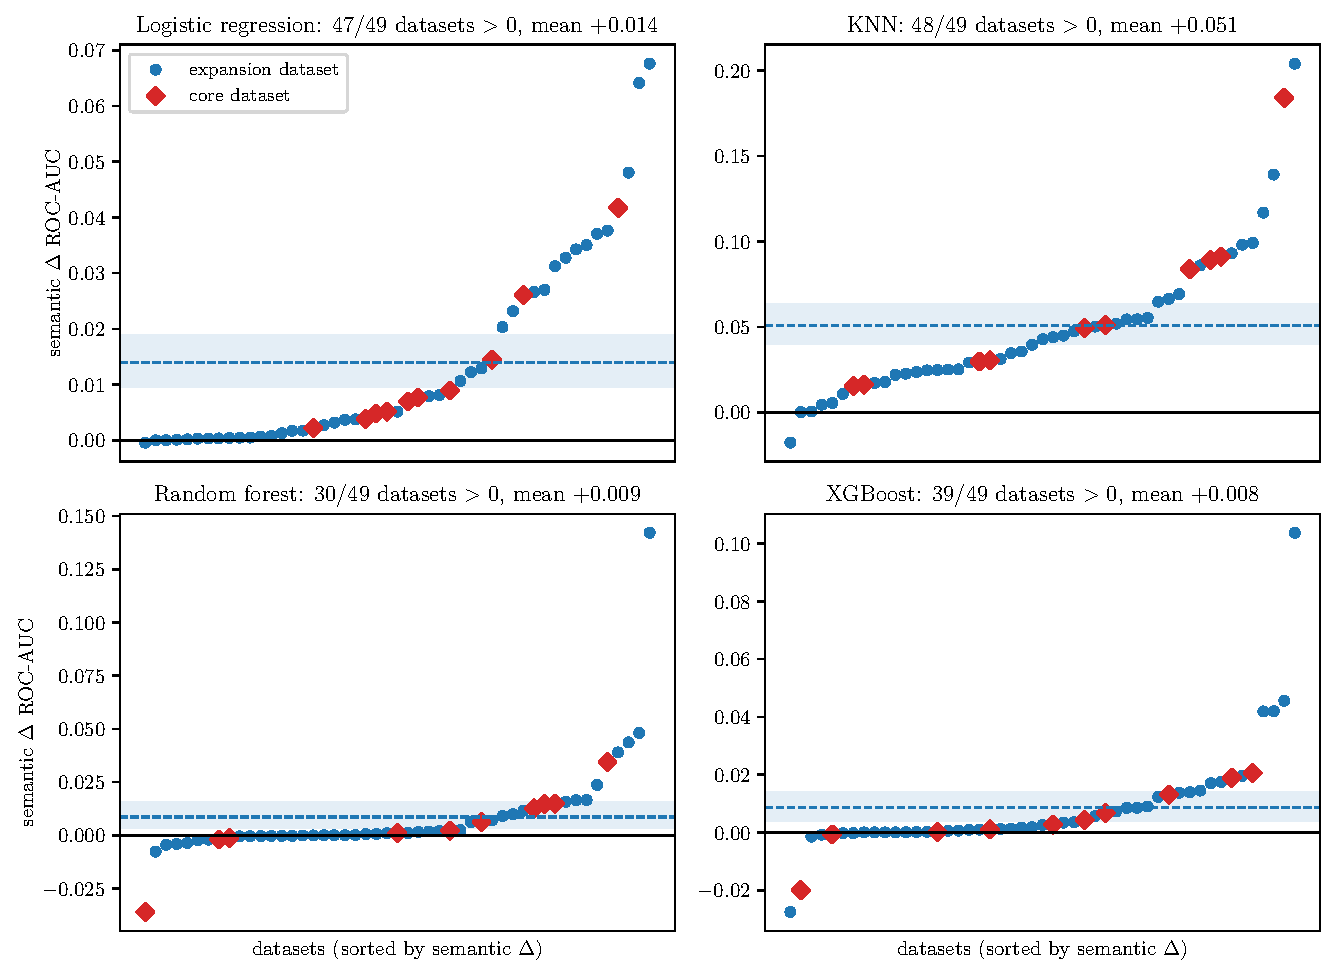
\includegraphics[width=0.92\linewidth]{figures/fig2_semantic_deltas.pdf}
\caption{Dataset-level semantic-control ROC-AUC deltas (\texttt{raw+formula} minus \texttt{raw+permuted-formula}) on all 49 datasets, one panel per downstream model, datasets sorted within each panel. Red diamonds are core datasets, blue dots expansion datasets; the dashed line is the mean and the band its 95\% bootstrap interval. The effect is positive on nearly every dataset for LR and KNN and on a clear majority for the tree ensembles.}\label{fig:semantic-dotplot}
\end{figure}


The result holds in each tier and without generator averaging. On the ten core datasets alone (linear/SVM schemas), LR and KNN are 10/0 (\(+0.012\) and \(+0.064\); nominal \(p = 0.002\)) and the tree ensembles positive in mean but not significant at \(N = 10\); on the 39 expansion datasets alone all four contrasts are significant (LR 37/1, KNN 38/1, RF 23/14 with \(p = 0.010\), XGBoost 31/5 with \(p = 5 \times 10^{-6}\)). On the 34 datasets covered by all four generators, LR is \(+0.018\) (34/0), KNN \(+0.054\) (33/1), RF \(+0.010\) and XGBoost \(+0.008\) (both \(p < 0.001\)). Each generator reproduces the pattern alone (Section~\ref{sec:generators}), as does averaging all three core-tier schema families (Appendix~\ref{app:core-families}).

Count-matched noise columns hurt every model (Table~\ref{tab:random-controls}, Appendix~\ref{app:extra-tables}), and \texttt{raw+formula} beats \texttt{raw+random-formula} for all four (LR \(+0.0134\), KNN \(+0.0541\), RF \(+0.0101\), XGBoost \(+0.0126\); Holm-corrected \(p < 0.001\)), so the gap is not a dimensionality artifact. One caveat: \(\Delta_{\mathrm{semantic}}\) is \(\Delta_{\mathrm{formula}}\) plus the harm permuted columns do relative to raw, roughly 30\% of the LR gap and most or all of the KNN, RF, and XGBoost gaps (permuted-minus-raw \(-0.044\), \(-0.007\), \(-0.009\) against direct gains \(+0.007\), \(+0.002\), \(0.000\)), so aligned columns are near-harmless and misaligned copies harmful, which shows that alignment matters but not that aligned formulas add information beyond raw features for the tree ensembles.

\subsection{How much of the semantic gap is generic? The random-expression control}\label{sec:random-expression}

Random valid expressions, the count-matched control of Section~\ref{sec:controls}, also beat their permuted copies for LR, KNN, and XGBoost (Table~\ref{tab:random-expression}; ROC-AUC: LR \(+0.0083\), 47/2; KNN \(+0.0391\), 48/1; XGBoost \(+0.0048\), 40/6; all Holm-corrected \(p < 0.001\)) and in mean for RF (\(+0.0031\), 29/18, \(p = 0.10\)). In mean this generic component is 59\% of the LLM semantic gap for LR, 77\% for KNN, 36\% for RF, and 57\% for XGBoost. The permutation control therefore certifies row alignment, not the quality of the generator's choices.

Two contrasts isolate those choices. First, random expressions add little: versus raw they help LR slightly (\(+0.0032\), 28/21, Holm-corrected \(p = 0.012\), a third of the LLM direct gain) and hurt KNN (\(-0.0068\), 9/40), RF (\(-0.0017\), 8/39), and XGBoost (\(-0.0007\), 14/32), against LLM direct gains of \(+0.0096\) (LR) and \(+0.0067\) (KNN) (Table~\ref{tab:semantic-direct}). Second, with both aligned, LLM formulas beat random expressions for LR (\(+0.0064\), 40/9, Holm-corrected \(p < 0.001\)), KNN (\(+0.0135\), 43/6, \(p < 0.001\)), and RF (\(+0.0036\), 31/16, \(p = 0.005\)), not for XGBoost (\(+0.0007\), 22/24); balanced accuracy agrees (RF \(+0.0069\), 32/16, \(p = 0.002\)). The excess semantic contrast (LLM minus random-expression) is positive and significant for all four models (\(+0.0037\) for XGBoost to \(+0.0118\) for KNN; Holm-corrected \(p < 0.001\) for LR, KNN, and RF, \(p = 0.003\) for XGBoost). The LLM-minus-random contrast holds for LR and KNN for each generator separately (uncorrected \(p \le 0.0008\) and \(p \le 0.0001\)) and on the 39 expansion datasets alone (LR \(+0.0073\), 32/7; KNN \(+0.0131\), 34/5); on the ten core datasets alone it is smaller (LR \(+0.0028\), 8/2, uncorrected \(p = 0.037\); KNN \(+0.0153\), 9/1, \(p = 0.004\)). Of the 8{,}400 random expression columns (five draws per cell), 29 were constant on the evaluation rows (15 cells); all were kept. The generator-specific signal is real but modest: about two fifths of the LLM permutation contrast for LR (\(0.0057/0.0140\)), a quarter for KNN (\(0.0118/0.0510\)), and, as a direct contrast, absent for XGBoost.


\begin{table}[tbp]
\caption{Random-expression control on all 49 datasets (ROC-AUC and balanced accuracy, generator-averaged). Each (dataset, generator) cell receives $k$ random but valid expressions over the dataset's own columns, drawn from the LLM formulas' vocabulary with design-split statistics only, where $k$ is the cell's number of LLM formula features (Section~\ref{sec:controls}); they are materialized, scored, and column-permuted exactly like the LLM formulas, and the random-expression columns of the table are averaged over five independent random schemas per cell. ``Random expr.\ $-$ raw'': \texttt{raw+random-expression} minus \texttt{raw}; ``Random expr.\ vs permuted'': random expressions minus their own permuted copy; ``LLM $-$ random expr.'': \texttt{raw+formula} minus \texttt{raw+random-expression}; ``Excess semantic'': the LLM semantic contrast of Table~\ref{tab:semantic-direct} minus the random-expression semantic contrast. W/L counts datasets (ties excluded); $p_{\mathrm{Holm}}$ is the exact Wilcoxon test over datasets, Holm-corrected over the four models.}\label{tab:random-expression}
\centering
\small
\begin{adjustbox}{max width=\linewidth}
\begin{tabular}{llrrrrrrrrrrrr}
\toprule
& & \multicolumn{3}{c}{Random expr. $-$ raw} & \multicolumn{3}{c}{Random expr. vs permuted} & \multicolumn{3}{c}{LLM $-$ random expr.} & \multicolumn{3}{c}{Excess semantic} \\
\cmidrule(lr){3-5}\cmidrule(lr){6-8}\cmidrule(lr){9-11}\cmidrule(lr){12-14}
Metric & Model & $\Delta$ & W/L & $p_{\mathrm{Holm}}$ & $\Delta$ & W/L & $p_{\mathrm{Holm}}$ & $\Delta$ & W/L & $p_{\mathrm{Holm}}$ & $\Delta$ & W/L & $p_{\mathrm{Holm}}$ \\
\midrule
ROC-AUC & Logistic regression & +0.0032 & 28/21 & 0.012 & +0.0083 & 47/2 & $<$0.001 & +0.0064 & 40/9 & $<$0.001 & +0.0057 & 39/10 & $<$0.001 \\
ROC-AUC & KNN & -0.0068 & 9/40 & $<$0.001 & +0.0391 & 48/1 & $<$0.001 & +0.0135 & 43/6 & $<$0.001 & +0.0118 & 38/11 & $<$0.001 \\
ROC-AUC & Random forest & -0.0017 & 8/39 & $<$0.001 & +0.0031 & 29/18 & 0.102 & +0.0036 & 31/16 & 0.005 & +0.0055 & 36/11 & $<$0.001 \\
ROC-AUC & XGBoost & -0.0007 & 14/32 & 0.008 & +0.0048 & 40/6 & $<$0.001 & +0.0007 & 22/24 & 0.778 & +0.0037 & 32/14 & 0.003 \\
\midrule
Bal. accuracy & Logistic regression & +0.0046 & 33/16 & 0.010 & +0.0101 & 46/3 & $<$0.001 & +0.0065 & 36/13 & 0.001 & +0.0064 & 37/12 & 0.002 \\
Bal. accuracy & KNN & -0.0094 & 10/38 & $<$0.001 & +0.0527 & 46/2 & $<$0.001 & +0.0218 & 41/7 & $<$0.001 & +0.0208 & 35/13 & $<$0.001 \\
Bal. accuracy & Random forest & +0.0007 & 19/28 & 0.183 & +0.0198 & 40/8 & $<$0.001 & +0.0069 & 32/16 & 0.002 & +0.0105 & 37/11 & $<$0.001 \\
Bal. accuracy & XGBoost & -0.0004 & 27/20 & 0.846 & +0.0093 & 42/5 & $<$0.001 & +0.0021 & 22/25 & 0.539 & +0.0044 & 33/14 & $<$0.001 \\
\bottomrule
\end{tabular}
\end{adjustbox}
\end{table}


\subsection{Direct formula gains are small and model-dependent}\label{sec:direct}

Direct gains over raw features are small and model-dependent (Table~\ref{tab:semantic-direct}, right half): LR gains \(+0.0096\) ROC-AUC (35/13, \(p = 1 \times 10^{-5}\), CI \(\lbrack +0.005, +0.015\rbrack\)) and KNN \(+0.0067\) (29/20, uncorrected \(p = 0.014\), Holm-corrected \(p = 0.042\)). The tree ensembles gain nothing: RF \(+0.0019\) (21/26, \(p = 0.39\)) and XGBoost \(0.0000\) (18/28, \(p = 0.52\)). Balanced accuracy agrees (Table~\ref{tab:semantic-direct}). The median LR gain is only \(+0.0027\): 13 of the 49 datasets gain more than \(+0.01\) and 12 more than \(+0.02\); most of the rest are within a few thousandths of zero, and two are negative (volcanoes \(-0.024\), employee turnover \(-0.016\)). The largest LR gains are bitcoinheist ransomware (\(+0.065\)), fried (\(+0.063\)), customer churn (\(+0.046\)), phoneme (\(+0.039\)), pol (\(+0.037\)), and jungle chess (\(+0.033\)). The direct LR gain holds in both tiers: \(+0.006\) on the ten core datasets (8/2, \(p = 0.010\)) and \(+0.010\) on the 39 expansion datasets (27/11, \(p < 0.001\)).

The LR gain is predictable: it concentrates where raw LR trails raw XGBoost (Spearman \(\rho = +0.69\), \(p = 4 \times 10^{-8}\) across the 49 datasets; \(\rho = +0.69\) for the semantic contrast as well). By tercile of that gap, from smallest to largest, the mean direct LR gain is \(+0.0003\) (median \(0.000\)), \(+0.004\), and \(+0.025\) (median \(+0.026\)); for KNN the correlation is \(\rho = +0.49\) (\(p < 0.001\)). Appendix~\ref{app:per-dataset} lists per-dataset deltas and Appendix~\ref{app:raw-scores} the raw-feature scores.

\subsection{Per-row judgments add no reliable value beyond formulas}\label{sec:per-row-judgments-add-no-reliable-value-beyond-formulas}

Table~\ref{tab:judgment} shows no reliable improvement from per-row judgments. All 120 core schema runs have a DeepSeek-Reasoner judgment matrix. For ROC-AUC, judgments add \(-0.0005\) to LR on average, \(+0.0016\) to RF, \(-0.0020\) to KNN, and \(+0.0002\) to XGBoost; on balanced accuracy every mean is below zero. Judgments win only 9 of 40 dataset-model ROC-AUC comparisons and 11 of 40 balanced-accuracy comparisons, and the one nominally significant cell (LR ROC-AUC, 1/9, \(p = 0.049\)) is in the unfavorable direction. The null is not an artifact of degenerate outputs: judgments alone are predictive (ROC-AUC 0.66 with logistic regression, Section~\ref{sec:scale-of-evaluation}) but add nothing to \texttt{raw+formula}, and a second judgment model gives the same null (Appendix~\ref{app:judgment-v4pro}). In a Friedman/Nemenyi ranking over the five core variants (CD \(= 1.93\) for \(k = 5\) and \(N = 10\)), \texttt{raw+formula+judgment} ranks below \texttt{raw+formula} for LR, KNN and XGBoost and above it for RF, always within the critical difference.


\begin{table}[tbp]
\caption{Incremental effect of per-row judgment features beyond deterministic formulas on the ten core datasets (12 schema runs per dataset, judgments by DeepSeek-Reasoner). $p$ is the exact two-sided Wilcoxon test over datasets; with $N = 10$ the smallest attainable $p$ is 0.002.}\label{tab:judgment}
\centering
\small
\begin{adjustbox}{max width=\linewidth}
\begin{tabular}{llrrrrr}
\toprule
Metric & Downstream model & \(N\) & Mean \(\Delta\) & W/L/T & Cliff's \(\delta\) & \(p\) \\
\midrule
ROC-AUC & Logistic regression & 10 & -0.0005 & 1/9/0 & -0.80 & 0.0488 \\
ROC-AUC & KNN & 10 & -0.0020 & 2/8/0 & -0.60 & 0.1309 \\
ROC-AUC & Random forest & 10 & +0.0016 & 5/5/0 & +0.00 & 0.8457 \\
ROC-AUC & XGBoost & 10 & +0.0002 & 1/9/0 & -0.80 & 0.0840 \\
\midrule
Bal. accuracy & Logistic regression & 10 & -0.0005 & 3/7/0 & -0.40 & 0.4316 \\
Bal. accuracy & KNN & 10 & -0.0031 & 3/7/0 & -0.40 & 0.1602 \\
Bal. accuracy & Random forest & 10 & -0.0009 & 3/7/0 & -0.40 & 0.1602 \\
Bal. accuracy & XGBoost & 10 & -0.0022 & 2/8/0 & -0.60 & 0.1055 \\
\bottomrule
\end{tabular}
\end{adjustbox}
\end{table}

Per-row judgments are the expensive part of the pipeline, and here that cost buys no measurable performance over formulas.

\subsection{Model-appropriate interaction}\label{sec:model-appropriate-interaction}

The model dependence is mechanistically plausible. Formula features are explicit basis expansions that a linear model cannot synthesize from raw inputs, so they enlarge the hypothesis class of logistic regression (Section~\ref{sec:direct}). Tree ensembles already build such interactions by recursive partitioning, and correlated formula columns can dilute a random forest's feature subsampling (\texttt{mtry} \(= \sqrt{p}\)) without adding information, consistent with its direct gain near zero. Hand-constructed interaction features on tic-tac-toe, MONK's Problem 1, and ionosphere illustrate this: LR gains \(+0.373\) ROC-AUC on tic-tac-toe while near-ceiling RF is unchanged (Appendix~\ref{app:mechanism}).

Critical-difference ranks agree (Figure~\ref{fig:cd}, Appendix~\ref{app:extra-tables}): with Nemenyi CD \(= 0.87\) over the five variants, \texttt{raw+formula} ranks first for LR (1.37, raw 1.90, within one CD) and second for XGBoost (2.03, raw 1.70), with the permuted and random controls more than one CD behind in both cases.

\subsection{Classical baselines}\label{sec:classical}

Three classical AutoFE baselines ran on exactly the DASEF protocol: pairwise polynomial interactions (top 12 by mutual information), OpenFE (top 12 generated features), and autofeat (log, square-root, and square transforms), each fitted with label access on the design split and materialized on the evaluation split. They keep 12 features, slightly more than the 9.7 to 10.2 LLM formulas per schema, and select them with labels; both favor the classical systems. Settings and coverage are in Appendix~\ref{app:extra-tables}.

Table~\ref{tab:classical} tests classical minus DASEF with a paired Wilcoxon test. The LLM formulas beat polynomial interactions for LR (ahead on 33 of 47 non-tied datasets, \(p = 0.005\)) and RF (\(p = 0.016\)) and are indistinguishable for KNN and XGBoost. They are indistinguishable from OpenFE for LR (21 wins to 25, \(p = 0.91\)), RF (\(p = 0.16\)) and XGBoost (\(p = 0.07\)), and OpenFE is ahead in mean for KNN (\(+0.0105\) versus \(+0.0069\), \(p = 0.056\); significant on balanced accuracy, Appendix~\ref{app:extra-tables}). They beat autofeat for LR on its 19 datasets (\(p = 0.029\)) and are indistinguishable otherwise. We therefore claim no superior generator: a strong classical search system is as good for LR and at least as good for KNN here; the formulas' distinguishing properties are zero inference cost, no label use, and human readability.

\begin{table}[tbp]
\caption{Classical automated-feature-engineering baselines on the 49-dataset benchmark: mean ROC-AUC deltas versus raw, with the generator-averaged DASEF formula deltas on the same datasets. Each classical system is fitted on the design split and applied to the evaluation split, so evaluation rows and label access match the DASEF protocol. W/L counts datasets on which the classical delta exceeds the DASEF delta; $p$ is the exact two-sided Wilcoxon test of classical minus DASEF.}\label{tab:classical}
\centering
\small
\begin{adjustbox}{max width=\linewidth}
\begin{tabular}{llrrrrr}
\toprule
Variant & Downstream model & \(N\) & Classical \(\Delta\) & DASEF formula \(\Delta\) & W/L (classical vs DASEF) & \(p\) \\
\midrule
Polynomial & Logistic regression & 49 & +0.0050 & +0.0096 & 14/33 & 0.005 \\
Polynomial & KNN & 49 & +0.0040 & +0.0067 & 21/28 & 0.235 \\
Polynomial & Random forest & 49 & -0.0022 & +0.0019 & 19/28 & 0.016 \\
Polynomial & XGBoost & 49 & -0.0003 & -0.0000 & 25/21 & 1.000 \\
\midrule
OpenFE & Logistic regression & 47 & +0.0110 & +0.0098 & 21/25 & 0.905 \\
OpenFE & KNN & 47 & +0.0105 & +0.0069 & 27/20 & 0.056 \\
OpenFE & Random forest & 47 & +0.0027 & +0.0019 & 30/16 & 0.160 \\
OpenFE & XGBoost & 47 & +0.0032 & +0.0003 & 29/16 & 0.069 \\
\midrule
autofeat & Logistic regression & 19 & +0.0130 & +0.0177 & 5/14 & 0.029 \\
autofeat & KNN & 19 & +0.0092 & +0.0120 & 8/11 & 0.395 \\
autofeat & Random forest & 19 & -0.0005 & +0.0006 & 7/12 & 0.332 \\
autofeat & XGBoost & 19 & -0.0003 & +0.0005 & 8/10 & 0.417 \\
\bottomrule
\end{tabular}
\end{adjustbox}
\end{table}

\subsection{Schema generator comparison}\label{sec:generators}

Each generator reproduces the pattern alone (Table~\ref{tab:generators}, Appendix~\ref{app:extra-tables}): the semantic control is significant for every generator and downstream model (uncorrected \(p < 0.05\); \(p < 0.001\) in 14 of 16 cells; LR means \(+0.013\) to \(+0.019\), KNN \(+0.048\) to \(+0.055\)). The direct LR gain is significant for every generator (\(+0.008\) to \(+0.014\), all \(p < 0.001\)), the direct KNN gain for three of four (Gemini excepted), and the tree ensembles gain nothing. No LLM dominates; per-generator ranges are narrower than dataset-to-dataset variation, and unequal dataset sets preclude a ranking.

\subsection{Replication on post-cutoff datasets}\label{sec:postcutoff}

Public OpenML tables leave open that the result reflects memorized feature recipes. We therefore repeat the analysis on six real Hugging Face tables published between March and May 2026, after the generators' training cutoffs (Appendix~\ref{app:postcutoff-data}), the longitudinal design used to measure contamination in code and reasoning benchmarks \citep{roberts2024cutoff,white2025livebench}. GPT-5.5 Pro and Gemini 3.1 Pro Preview each generate all three schema families, averaged per dataset before testing; 35 of the 36 planned runs (six datasets \(\times\) two generators \(\times\) three families) completed; the GPT-5.5 Pro tree-family cell on prediction markets timed out after three attempts. Appendix~\ref{app:extra-tables} gives settings, cutoffs, and scope.

The semantic control replicates (Table~\ref{tab:postcutoff}): formulas beat their permuted copies for every downstream model, 6/0 (\(p = 0.031\), the smallest attainable two-sided \(p\) at \(N = 6\)) for LR and XGBoost on ROC-AUC and for LR, KNN, and XGBoost on balanced accuracy, 5/1 otherwise; the direct LR gain is also 6/0 (\(+0.042\) ROC-AUC, \(+0.040\) balanced accuracy, \(p = 0.031\)). Prediction markets dominate (LR \(+0.19\), KNN \(+0.31\) ROC-AUC, permuted contrast); without them (\(N = 5\), smallest attainable \(p\) 0.063) the permuted contrast stays positive for all four models (ROC-AUC: LR \(+0.014\), 5/0; RF \(+0.003\), 4/1; KNN \(+0.029\), 4/1; XGBoost \(+0.005\), 5/0), nothing reaches \(p < 0.05\), and the direct LR gain falls from \(+0.042\) to \(+0.015\). Three targets are weak by construction: 62.5\% of prediction-market rows have open equal to high with none labeled up, and high minus open alone reaches ROC-AUC 0.93, a within-row bookkeeping identity; two retained sponsor-type flags alone reach ROC-AUC 0.78 on clinical trials; and 97\% of real-estate rows duplicate another row except for the scrape-time code, and water-quality samples share site covariates, making row-wise cross-validation optimistic. This is a supportive replication, not a powered confirmation.

\begin{table}[tbp]
\caption{Post-cutoff replication: dataset-level mean deltas over six real datasets whose public tables post-date the generators' training data (Appendix~\ref{app:postcutoff-data}); all three schema families of both generators are averaged per dataset. ``Semantic $\Delta$'' is \texttt{raw+formula} minus \texttt{raw+permuted-formula}, the same column-permutation control as Table~\ref{tab:semantic-direct}. ``Direct $\Delta$'' is \texttt{raw+formula} minus \texttt{raw}. With $N = 6$ the minimum two-sided Wilcoxon $p$ is 0.031 (6/0).}\label{tab:postcutoff}
\centering
\small
\begin{adjustbox}{max width=\linewidth}
\begin{tabular}{llrrrrrr}
\toprule
Metric & Downstream model & Semantic \(\Delta\) & W/L & \(p\) & Direct \(\Delta\) & W/L & \(p\) \\
\midrule
ROC-AUC & Logistic regression & +0.0436 & 6/0 & 0.0312 & +0.0418 & 6/0 & 0.0312 \\
ROC-AUC & Random forest & +0.0169 & 5/1 & 0.1562 & +0.0119 & 4/2 & 0.3125 \\
ROC-AUC & KNN & +0.0762 & 5/1 & 0.0625 & +0.0119 & 4/2 & 0.4375 \\
ROC-AUC & XGBoost & +0.0185 & 6/0 & 0.0312 & +0.0159 & 4/2 & 0.2188 \\
\midrule
Bal. accuracy & Logistic regression & +0.0421 & 6/0 & 0.0312 & +0.0401 & 6/0 & 0.0312 \\
Bal. accuracy & Random forest & +0.0373 & 5/1 & 0.0625 & +0.0159 & 3/3 & 1.0000 \\
Bal. accuracy & KNN & +0.0777 & 6/0 & 0.0312 & +0.0178 & 4/2 & 0.8438 \\
Bal. accuracy & XGBoost & +0.0339 & 6/0 & 0.0312 & +0.0297 & 4/2 & 0.3125 \\
\bottomrule
\end{tabular}
\end{adjustbox}
\end{table}

\subsection{Anonymized-column control}\label{sec:anon}

To test whether the effect depends on recognizing the columns at all, we regenerate linear/SVM schemas with GPT-5.5 Pro on an anonymized view of the 10 core datasets, replacing column, dataset, and target names by generic tokens (\texttt{x001}, \texttt{x002}, \ldots) and retaining the distributional summary (contents and remaining identity cues in Appendix~\ref{app:extra-tables}), and re-run the controls. Hiding names and identity should remove any effect built on memorized recipes for these named datasets.

It does not (Table~\ref{tab:anon}). The semantic control survives for the capacity-limited models, LR ROC-AUC \(+0.011\) (10/0, \(p = 0.002\)) and KNN \(+0.070\) (10/0, \(p = 0.002\)), comparable to GPT-5.5 Pro's named-column result (LR \(+0.009\), 10/0; KNN \(+0.064\), 9/1); on balanced accuracy it is 10/0 for RF, KNN, and XGBoost (\(p = 0.002\)) and 9/1 for LR (\(p = 0.004\)). One cell is not row-identical: anonymized phoneme used the 5,000-row cap (3,500 rows), not the uncapped 3,783 rows, and its raw LR score differs by 0.009. Against count-matched random expressions on the same ten cells (Section~\ref{sec:random-expression}), anonymized formulas are better for KNN (\(+0.020\), 10/0, \(p = 0.002\)) but not reliably for LR (\(+0.002\), 7/3, \(p = 0.11\)), and named formulas likewise (KNN \(+0.014\), 8/2, \(p = 0.037\); LR \(+0.000\), 8/2, \(p = 0.23\)), so we claim no generator-specific LR signal on the core tier. The row-aligned component therefore does not require recognizing the dataset or its columns; much of it is generically sensible algebra (ratios, products, thresholds), and the generator-specific KNN component survives anonymization. With the post-cutoff replication, this points to domain-agnostic feature-engineering heuristics plus a column-name-independent generator-specific component for the capacity-limited models, not memorized benchmark knowledge; the LLM is not acting as a domain expert.

\begin{table}[tbp]
\caption{Anonymized-column control (10 core datasets; linear/SVM schemas from GPT-5.5 Pro; column names and dataset identity hidden). ``Semantic $\Delta$'' is \texttt{raw+formula} minus \texttt{raw+permuted-formula}; ``Direct $\Delta$'' is \texttt{raw+formula} minus \texttt{raw}. The semantic effect survives anonymization for LR and KNN.}\label{tab:anon}
\centering
\small
\begin{adjustbox}{max width=\linewidth}
\begin{tabular}{llrrrr}
\toprule
Metric & Downstream model & Direct \(\Delta\) & Semantic \(\Delta\) & Sem. W/L & Sem. \(p\) \\
\midrule
ROC-AUC & Logistic regression & +0.0048 & +0.0110 & 10/0 & 0.0020 \\
ROC-AUC & KNN & +0.0087 & +0.0699 & 10/0 & 0.0020 \\
ROC-AUC & Random forest & -0.0001 & +0.0060 & 8/2 & 0.1309 \\
ROC-AUC & XGBoost & -0.0006 & +0.0037 & 7/3 & 0.1934 \\
\midrule
Bal. accuracy & Logistic regression & +0.0077 & +0.0182 & 9/1 & 0.0039 \\
Bal. accuracy & KNN & +0.0338 & +0.1097 & 10/0 & 0.0020 \\
Bal. accuracy & Random forest & +0.0081 & +0.0625 & 10/0 & 0.0020 \\
Bal. accuracy & XGBoost & +0.0033 & +0.0328 & 10/0 & 0.0020 \\
\bottomrule
\end{tabular}
\end{adjustbox}
\end{table}

\section{Discussion}\label{sec:discussion}

\paragraph{The semantic-control result is the anchor.}

Aligned formula features beat their row-permuted copies, significantly after correction for all four downstream models on 49 datasets, for each generator alone, and in both tiers. The random-expression control (Section~\ref{sec:random-expression}) sets the scale: valid expressions of any origin beat their permuted copies, roughly three fifths of the permutation contrast for LR and three quarters for KNN. The generator-specific remainder (\(+0.006\) for LR, \(+0.014\) for KNN, \(+0.004\) for RF) is significant, consistent across generators, and absent for XGBoost. Reproduction on six post-cutoff datasets (Section~\ref{sec:postcutoff}) and under anonymization (Section~\ref{sec:anon}) makes memorized recipes unlikely.

\paragraph{Direct predictive gains are real but small.}

For LR the raw-to-formula gain is significant on 49 datasets but its median is a quarter of a point of ROC-AUC; for KNN it is smaller (\(+0.007\), Holm-corrected \(p = 0.042\)); for the tree ensembles it is absent. The OpenFE comparison (Table~\ref{tab:classical}) shows that row-aligned structure does not make the formulas the best available generator; the claim is mechanistic.

\paragraph{Per-row judgments are not worth their cost here.}

Formula generation is one schema call per dataset and generator, roughly \$0.03 to \$0.50 per call at list prices by generator from measured token usage. Judgment generation needs inference over every evaluation row: 21 to 152 batched calls per dataset and schema (25 rows per call, 524 to 3,783 evaluation rows), roughly \$0.06 to \$5 per dataset with DeepSeek-Reasoner at list prices. That multiplier reaches one to two orders of magnitude on the larger datasets and buys no measurable performance over formulas. Prefer formulas unless a separate validation set shows a clear judgment-feature gain.

\paragraph{Downstream-awareness as a reusable protocol.}

Prompting for linear/SVM, tree, or distance-based model families did not reliably produce better-matched features. On the core tier the matched family beat the better mismatched family in only 57 of 160 ROC-AUC comparisons (44 of 120 for LR, RF, and KNN; 48 of 160 on balanced accuracy), consistent with the one-third expected under the null (Appendix~\ref{app:extra-tables}). This is a diagnostic null; the protocol is documented for reuse.

\paragraph{Implications for benchmarking LLM data-preparation tools.}

The protocol transfers to any tool that rewrites a tabular feature representation. It rests on count-matched and random-expression controls (Section~\ref{sec:controls}), dataset-level tests (Section~\ref{sec:statistical-analysis}), and contamination checks (Sections~\ref{sec:postcutoff} and~\ref{sec:anon}). Its inputs are pinned: OpenML identifiers, versions, licences, and source repositories (Appendices~\ref{app:postcutoff-data} and~\ref{app:datasets}), and generator responses cached by prompt hash (Section~\ref{sec:scale-of-evaluation}). The benchmark and controls are released so that other generators can be scored on the same footing.

\subsection{Limitations}\label{sec:limitations}

First, formula-mechanism claims rest on 49 datasets, but the judgment null, family diagnostic, and anonymized control rest on ten core datasets (DeepSeek-V4-Pro gives the same null on 93 runs; Appendix~\ref{app:judgment-v4pro}). Second, the expansion tier covers only the linear/SVM family; agreement among families (Appendix~\ref{app:core-families}) was verified only on the core tier. Third, contamination of public OpenML tables cannot be fully ruled out: the post-cutoff set (Section~\ref{sec:postcutoff}) has six datasets with known weaknesses, and the anonymized schemas (Section~\ref{sec:anon}) used one model and kept class-label strings. Fourth, only classification is included, and nine of 49 datasets have raw XGBoost above ROC-AUC 0.995, leaving no room for gains. Fifth, the semantic effect is modest (median ROC-AUC \(\Delta\) roughly \(+0.001\) to \(+0.04\) by model); the claim is existence and direction, not magnitude. Sixth, the AutoFE comparison covers three classical systems, not LLM-search methods such as CAAFE. Seventh, for three core datasets the schema generators received the categorical columns as integer codes (Section~\ref{sec:protocol}), so their formulas operate on arbitrary codes; the downstream models receive these columns one-hot encoded. Eighth, one schema per cell leaves unmeasured schema-sampling variance in generator comparisons. Ninth, the random-expression control averages five uniform draws per cell from a fixed two-column vocabulary; label-free search over it might narrow the gap (Appendix~\ref{app:extra-tables}). Tenth, the 5,000-row cap means tree-ensemble baselines are not full-data baselines and the small LR gains are untested at full scale.

\section{Conclusion}\label{sec:conclusion}

LLM-generated deterministic formulas carry row-aligned signal: they beat the same features with generated columns independently permuted across rows. On 49 OpenML datasets it is significant after correction for all four downstream models and all four generators, survives anonymization, and replicates in direction on six real post-cutoff tables. Semantic signal is not state-of-the-art prediction: direct gains are small for LR and KNN, concentrated where raw linear models trail gradient boosting, and absent for tree ensembles; OpenFE is as good for LR and at least as good for KNN; per-row judgments add nothing reliable beyond zero-inference-cost formulas. Use LLMs, if at all, for cheap, interpretable, schema-level formulas validated against raw, AutoFE, and gradient-boosted-tree baselines. Evaluating such tools needs count-matched, row-permutation, and random-expression controls, post-cutoff or anonymized tables, and documented provenance, versions, and licences. Code, schemas, and scores are released.
